%%% File encoding: UTF-8
%% äöüÄÖÜß  <-- no German Umlauts here? Use an UTF-8 compatible editor!

%%% Magic comments for setting the correct parameters in compatible IDEs
% !TeX encoding = utf8
% !TeX program = pdflatex 
% !TeX spellcheck = de_DE
% !BIB program = biber

\documentclass[master,german]{hgbthesis}
% Permissible options in [..]: 
%   Type of work: diploma, master (default), bachelor, internship 
%   Main language: german, english (default)
%%%----------------------------------------------------------

\RequirePackage[utf8]{inputenc}		% Remove when using lualatex or xelatex entfernen!
\usepackage{graphicx}
\usepackage{svg}
\usepackage{minted}
\usepackage{listings}
\usepackage{varioref}
\usepackage{longtable}
\usepackage{tabularx}
\geometry{top=2.5cm,left=3.5cm,bottom=2.5cm,right=3.5cm}

% -----------------------------------------------------
\newenvironment{code}{\captionsetup{type=listing}}{}
% -----------------------------------------------------
% -----------------------------------------------------
\newcommand{\mysubsubsection}[1]{{\subsubsection{\textbf{#1}}}}
\newcommand{\mentionedtext}[1]{{\textit{{#1}}}}
\newcommand{\sourceDir}{./sources}
\newcommand{\sourceFontSize}{\fontsize{10pt}{11.5}}
\newcommand{\quotes}[1]{``#1''}
\newmintedfile[bashFile]{bash}{
	linenos=false, 
	frame=none, 
	breaklines=true, 
	tabsize=2,
	numbersep=5pt,
	xleftmargin=10pt,
	baselinestretch=1,
	fontsize=\sourceFontSize
}
\newmintedfile[yamlFile]{yaml}{
	linenos=false, 
	frame=none, 
	breaklines=true, 
	tabsize=2,
	numbersep=5pt,
	xleftmargin=10pt,
	baselinestretch=1,
	fontsize=\sourceFontSize
}
\newmintedfile[javaFile]{java}{
	linenos=false, 
	frame=none, 
	breaklines=true, 
	tabsize=2,
	numbersep=5pt,
	xleftmargin=10pt,
	baselinestretch=1,
	fontsize=\sourceFontSize
}
\newmintedfile[xmlFile]{xml}{
	breaklines=true, 
	tabsize=2,
	numbersep=5pt,
	xleftmargin=10pt,
	baselinestretch=1,
	autogobble=true,
	breakautoindent=false,
	fontsize=\sourceFontSize
}
\newmintinline[inlineJava]{java}{
	fontsize=\sourceFontSize
}
\newmintinline[inlineBash]{bash}{
	fontsize=\sourceFontSize
}
% -----------------------------------------------------
\graphicspath{{images/}}    % location of images and graphics
\logofile{logo}				% logo file = images/logo.pdf (use \logofile{} for no logo)
\bibliography{references.bib}  	% name of bibliography file (references.bib)
\setlength{\parindent}{0pt}
\usepackage{titlesec}

\titleformat{\section}[display]
{\normalfont\bfseries}{}{0pt}{\Huge}

\renewcommand*{\labelalphaothers}{}
\DeclareLabelalphaTemplate{
	\labelelement{
		\field[final]{shorthand}
		\field{labelname}
		\field{label}
	}
	\labelelement{
		\literal{,\addhighpenspace}
	}
	\labelelement{
		\field{year}
	}
}
%%%----------------------------------------------------------
% Title page entries
%%%----------------------------------------------------------

%%% Entries for ALL types of work: --------------------------
\title{Implementierung einer Partnerdatenbank und Evaluierung des verwendeten Technologiestack} %no camel used (and Camel)
%\author{Ing. Thomas Herzog B.Sc}
%\programname{Software Engineering}
\placeofstudy{Hagenberg}
\dateofsubmission{2020}{05}{30}	% {YYYY}{MM}{DD}

%%% Entries for Bachelor theses only: -----------------------
%\thesisnumber{XXXXXXXXXX-A}   %e.g. 1310238045-A  
% (Stud-ID, A = 1st Bachelor thesis)
%\semester{Fall Semester 2017} 	% Fall/Spring Semester YYYY
%\coursetitle{Introduction to Trivial Problems 1} 
\advisor{FH-Prof. DI Dr. Herwig Mayr}

%%% Restricted publication license instead of CC (master only):
%\cclicense

%%%----------------------------------------------------------
\begin{document}
%%%----------------------------------------------------------

%%%----------------------------------------------------------
\frontmatter							% title part (roman page numbers)
%%%----------------------------------------------------------

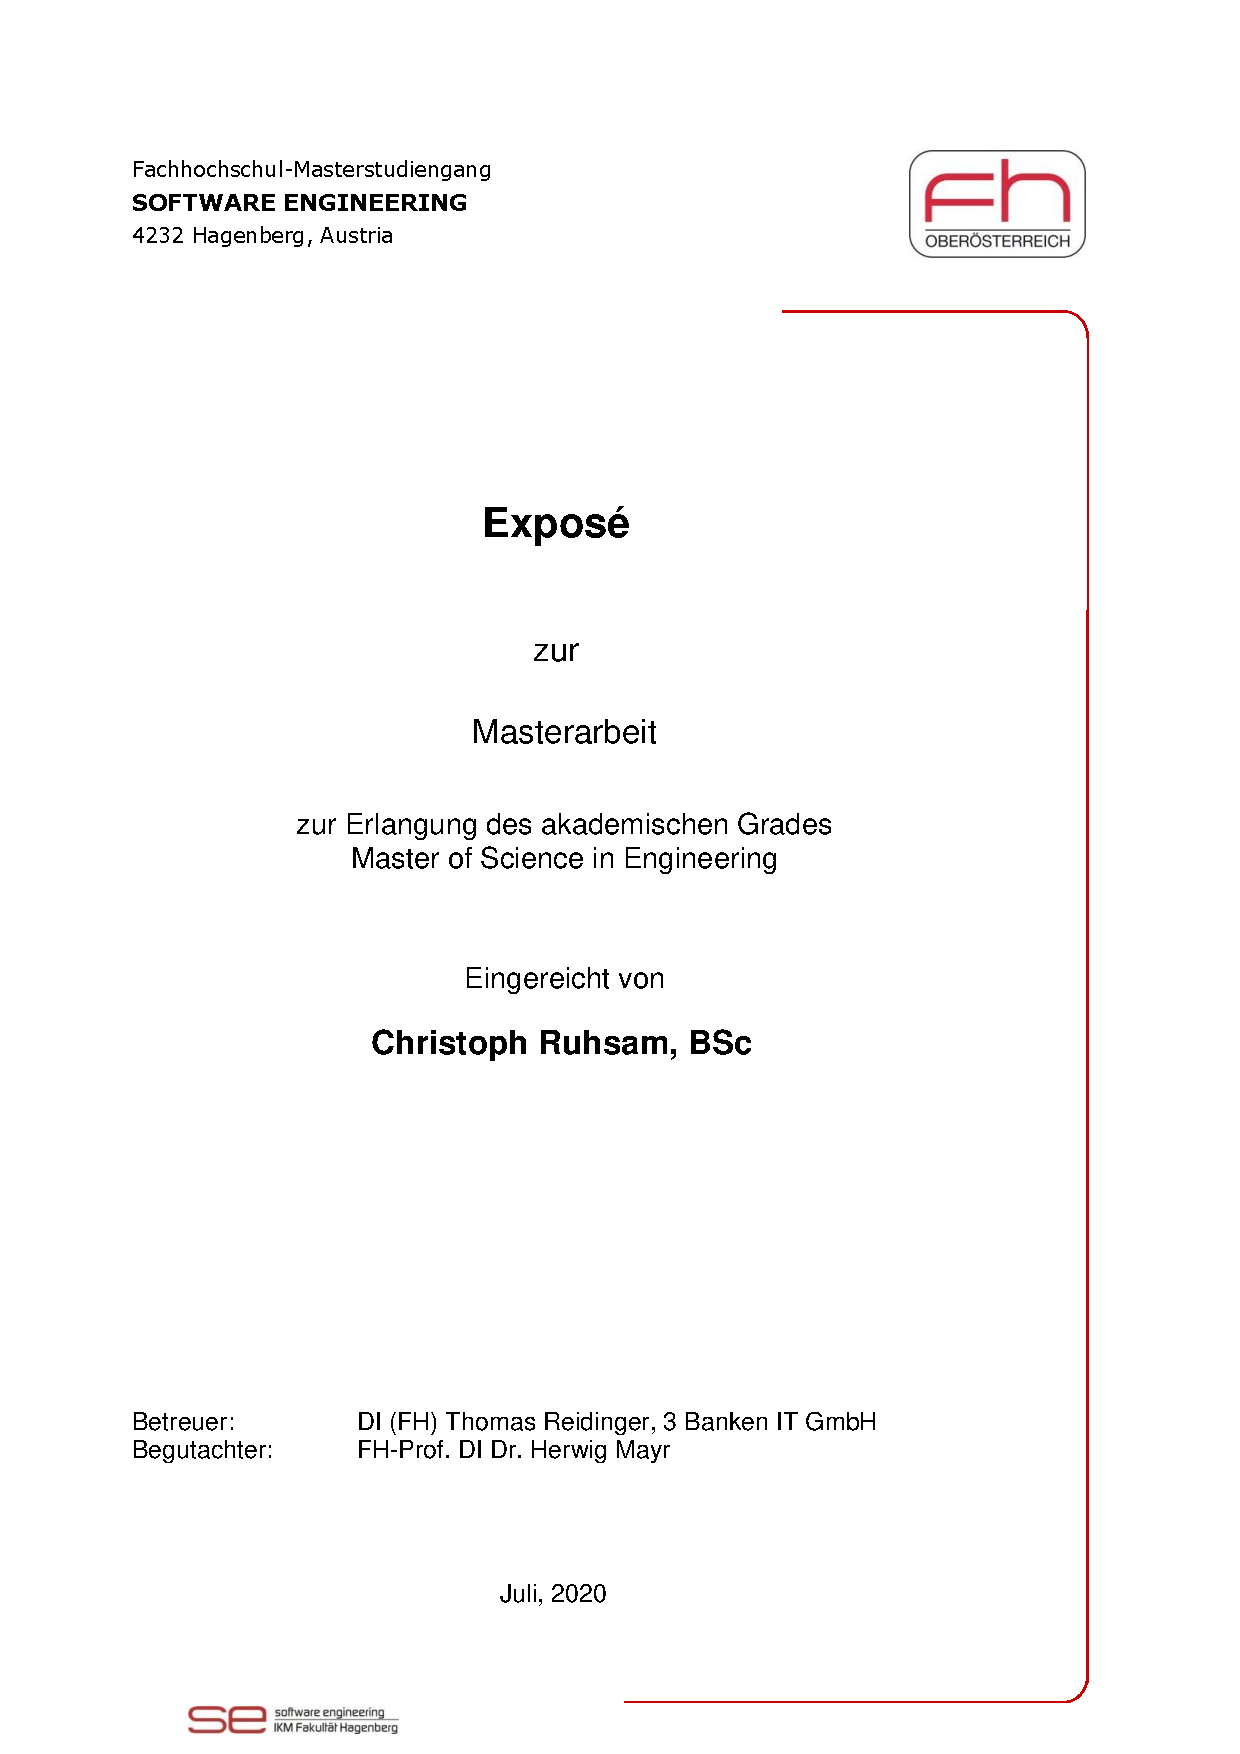
\includepdf{title.pdf}
%\maketitle
%\tableofcontents

%\chapter{Preface}






 	% preface is optional
%\chapter{Abstract}
An Enterprise Service Bus (ESB) is a crucial part of an enterprise, which connects the enterprise to its partners, customers, and other branches. The appearance of containerization, cloud services, and the microservice architecture have provided new possibilities for implementing and running an ESB. But, an ESB is commonly used by large conservative enterprises, which don't adapt new technologies fast, and wait until a new technology has proven itself. Especially the cloud is something the industry denied to use for a long time, because of the fact, that the infrastructure and data are managed and maintained by external service providers. \\ 

These days, we live in the so called cloud age, whereby global enterprises like Red Hat or Amazon provide cloud services such as Platform as a Service (PaaS), which can scale with the business. Enterprises start to consider to move their ESB installations to the cloud to profit from the cloud service provided features. Moving an ESB to the cloud will be a long term process for an enterprise, because the established processes for development, running, and managing the ESB will have to change. \\

This thesis has the goal to give the reader an overview of the cloud related concepts and technologies such as, Infrastructure as Code (IaC) and Docker, which are the base for cloud services. The implemented ESB prototype,  is  available at \url{https://github.com/cchet-thesis-msc/prototype}, and shows how an ESB could be implemented on a PaaS platform. \\




%%%----------------------------------------------------------
\mainmatter          			% main part (arabic page numbers)
%%%----------------------------------------------------------

\section{Titel der finalen Arbeit}
Die 3 Banken IT GmbH möchte zur Verwaltung ihrer Parnter ein einheitliches System. Derzeit werden Partner in verschiedenen Systemen (z.B. SAP, Excel-Liste, Word-Dokument) abgelegt. Es soll eine Partnerdatenbank implementiert werden, die das Verwalten der Partner vereinfacht.
Der Titel der finalen Arbeit lautet daher: \glqq \textbf{Implementierung einer Partnerdatenbank und Evaluierung des verwendeten Technologiestacks}\grqq.

{\let\clearpage\relax \section{Motivation und Ziel}}
Ziel dieser Arbeit ist die Erleichterung der Partnerverwaltung für die 3 Banken IT GmbH, sowie die Erlangung von Wissen und Erfahrung des Autors mit den verwendeten Technologien. Auch die Evaluierung der verwendeten Technologien wird als Ziel definiert, sodass der Autor in zukünftigen Projekten selbst die passende Technologie für verschiedene Anwendungsgebiete wählen kann.

Dies ist zugleich die Motivation der Arbeit. Der Autor soll ein breit gefächertes Wissen über die aktuell vorhandenen und in der Praxis verwendeten Technologien erlangen und selbständig die Passendste für das jeweilige Projekt auswählen können.

\section{Unternehmen}
Die 3 Banken IT GmbH ist der IT-Dienstleister der 3-Banken-Gruppe. Zur 3-Banken-Gruppe gehören die drei Regionalbanken Oberbank AG, Bank für Tirol und Vorarlberg AG und die BKS Bank AG.
Die Geschäftsführer der 3 Banken IT GmbH sind Karl Stöbich, MBA und Mag. Alexander Wiesinger, MBA. Der Standort ist in Linz.
Das Dienstleistungsspektrum der 3 Banken IT GmbH umfasst: \newline
\begin{enumerate}
	\item Applikationsentwicklung/Banken-Lösungen
	\item IT - Security
	\item Rechenzentrums– und IT-Infrastruktur-Dienstleistungen und
	\item Outputservice \& ZV-Abwicklung \newline
\end{enumerate} 

In der Zentrale Linz und in den beiden Kompetenzzentren in Klagenfurt und Innsbruck sind derzeit 254 Mitarbeiter beschäftigt.
\cite{3BankenIT}

\section{konkrete Aufgabenstellung}
Die konkrete Aufgabenstellung ist die Implementierung einer Partnerdatenbank zur erleichterten Verwaltung der Partner. Zu den Partnern der 3 Banken IT GmbH zählen unter anderem die FH Oberösterreich, die Studiengesellschaft für Zusammenarbeit im Zahlungsverkehr GmbH, die Christian Doppler Forschungsgesellschaft, etc.
Derzeit werden die Partner in unterschiedlichen Systemen gehalten und verwaltet. Dazu zählen SAP, eine Excel-Liste und unterschiedliche Kontaktdaten, die bei den Mitarbeitern selbst gehalten werden.

Die Technologien für die Applikation werden von der 3 Banken IT GmbH festgelegt und sind\newline
\begin{enumerate}
	\item eine Microsoft SQL Datenbank,
	\item Springboot als Backend
	\item und Angular als Frontend. \newline 
\end{enumerate}


Dazu soll mindestens der Erstkontakt, also die Aufnahme der Kontaktdaten des Partners, die graphische Darstellung der jeweiligen Partner, sowie die Kündigung und Löschung der Daten implementiert werden.

Auch die Evaluierung der verwendeten Technologien in Bezug auf Vor- und Nachteile und Alternativen gehört zu den Aufgaben der Arbeit.

\section{Vorgehensweise}
Die Vorgehensweise erfolgt inkrementell. Der Autor beschreibt während der Implementierung des Systems die wichtigsten Abschnitte in der Arbeit und nicht erst nach Fertigstellung der Applikation.
Bei der Applikationsentwicklung werden mit der 3 Banken IT GmbH Teilabschnitte ausgemacht, bis wann, welche Funktionen fertiggestellt sein sollen, bzw. welche Features noch eingebaut werden können. Die Applikation selbst soll bis Ende Mai fertiggestellt und der 3 Banken IT GmbH übergeben werden.
\newline \newline
Zur Erstellung der Schrift wird zu Beginn ein Inhaltsverzeichnis inklusive Schätzungen der Seitenzahlen abgegeben. Danach wird mt dem Betreuer ein Probekapitel ausgemacht, das fertiggestellt wird und dem Betreuer zur Durchsicht abgegeben wird. Dies dient als Orientierung zum Verfassen der finalen Schrift. Die finale Schrift soll bist spätestens Anfang Mai 2020 fertiggestellt sein, damit ein Antreten bei dem ersten Termin der Masterprüfung möglich ist.

\section{Organisatorische Details}
Die Schrift wird in Deutsch gehalten.
Die fertige Schrift wird auch der 3 Banken IT GmbH zur Durchsicht gegeben. Die 3 Banken IT GmbH entscheidet über die Sperre der Schrift, sofern firmeninterne oder vertrauliche Daten beschrieben werden. Der Autor der Schrift besteht nicht auf die Sperre der Arbeit.

\section{Wichtige Meilensteine}
Die nachfolgende Tabelle gibt einen Überblick über die wichtigsten Meilensteine der Arbeit.
\begin{table}[H]
%	\resizebox{\textwidth/2}{!}{%
		\begin{tabular}{ll}
			\hline
			\multicolumn{1}{|l|}{Datum} & \multicolumn{1}{l|}{Aufgabe} \\ \hline
			\multicolumn{1}{|l|}{2019-11-15} & \multicolumn{1}{l|}{Abgabe des Inhaltsverzeichnisses} \\ \hline
			\multicolumn{1}{|l|}{2020-01-10} & \multicolumn{1}{l|}{Abgabe des Probekapitel} \\ \hline
			\multicolumn{1}{|l|}{2020-05-01} & \multicolumn{1}{l|}{Abgabe des Literaturverzeichnisses} \\ \hline
			\multicolumn{1}{|l|}{2020-05-08} & \multicolumn{1}{l|}{Abgabe der finalen Schrift} \\ \hline
			\multicolumn{1}{|l|}{2020-05-30} & \multicolumn{1}{l|}{Übergabe des Prototypen} \\ \hline
		\end{tabular}%
%	}

\end{table}

\section{Wichtige Literatur}
Im folgenden wird die wichtigste Literatur der Arbeit dargestellt.
\begin{enumerate}
	\item \cite{SpringBoot2}: Spring Boot 2 ist die verwendete Backend-Technologie. Das Buch \citetitle{SpringBoot2} wird benötigt, um diese Technologie zu beschreiben.
	\item \cite{ProAngular6}: Angular wird als Frontend-Technologie verwendet. \citetitle{ProAngular6} dient zum Beschreiben dieser Technologie.
	\item \cite{3BankenIT}: Zur Beschreibung des Unternehmens wird die Firmenhomepage verwendet. 
	\item \cite{FullStackReact}: Auch ein Vergleich des verwendeten Technologiestacks mit Ähnlichen ist Thema der Arbeit. ReactJS ist eine Frontend-Technologie. Das Buch \citetitle{FullStackReact} dient zum Evaluieren der Vor- und Nachteile von ReactJS und dem Vergleich mit Angular.
	\item \cite{JavaEE}: JavaEE ist eine ähnliche Technologie zu Spring Boot. Das Buch \citetitle{JavaEE} dient ebenfalls zum Vergleich der Vor- und Nachteile.
\end{enumerate}

%%%----------------------------------------------------------
\MakeBibliography                     				% references
%%%----------------------------------------------------------
%%% special page for checking print size --------------------
%\chapter*{Check Final Print Size}

\begin{center}
{\Large --- Check final print size! ---}

\bigskip

\calibrationbox{100}{50} % width/height of box in mm

\bigskip

{\Large --- Remove this page after printing! ---}

\end{center}



%%%----------------------------------------------------------
\end{document}
%%%----------------------------------------------------------